\documentclass{deliverablereport}
\usepackage{pdfpages}

\usepackage[style=alphabetic,backend=bibtex]{biblatex}
\addbibresource{../../lib/kbibs/kwarcpubs.bib}
\addbibresource{../../lib/kbibs/extpubs.bib}
\addbibresource{../../lib/kbibs/kwarccrossrefs.bib}
\addbibresource{../../lib/kbibs/extcrossrefs.bib}
\addbibresource{../../lib/deliverables.bib}
%\addbibresource{../../lib/publications.bib}
\addbibresource{rest.bib}
% temporary fix due to http://tex.stackexchange.com/questions/311426/bibliography-error-use-of-blxbblverbaddi-doesnt-match-its-definition-ve
\makeatletter\def\blx@maxline{77}\makeatother

\deliverable{component-architecture}{scscp-sage}
\deliverydate{02/27/2017}
\duedate{02/27/2017 (Month 18)}
\def\pn{OpenDreamKit}
\author{ }

\begin{document}
\maketitle
%  Work Package WP6 develops a novel, foundational, knowledge-based framework for
  interfacing existing open source mathematical software systems and knowledge bases into
  a mathematical VRE, where systems can delegate functionalities among each other
  seamlessly without losing semantics.

  The overall Math-in-the-Middle (MitM) Framework developed in WP6 over the last three
  years is described in D6.5; this Report complements it by describing the curated
  contents Math-in-the-Middle (MitM) Ontology which serves as a reference and pivotal
  point for translations between the various input languages of mathematical software
  systems and knowledge bases.

  In a nutshell, the MitM Ontology describes the mathematical objects, concepts, and their
  relations in a general, system-agnostic way in an OMDoc/MMT theory graph while the
  mathematical systems export API theories that describe the system interface language in
  terms of types, classes, constructors, and functions -- again in OMDoc/MMT. These two
  levels of descriptions are linked by OMDoc/MMT alignments that allow the translation of
  expressions between systems.

%%% Local Variables:
%%% mode: visual-line
%%% fill-column: 5000
%%% mode: latex 
%%% TeX-master: "report"
%%% End:

% TODO: update GitHub issue description
\strut\githubissuedescription
\newpage\tableofcontents\newpage

\section{Introduction}\label{intro}

{\sf SCSCP} stands for the 
{\bf Symbolic Computation Software Composability Protocol}
-- a remote procedure call framework by which different
software components (primarily mathematical software systems) 
may offer computational services to a variety of possible
clients, such as, for example:
\begin{itemize}
\item a computer algebra system (CAS) running on the same computer system or remotely;
\item another instance of the same CAS (in a parallel computing context);
\item a simplistic SCSCP client (e.g. C/C++/Python/etc. program) with a minimal 
SCSCP support needed for a particular application;
\item an internet application providing user interface to the computational services;
\item a Web server which passes on the same services as Web services to other applications;
\item Cloud middleware
\end{itemize}
using the OpenMath encoding (see \url{http://www.openmath.org/})
both for the data and protocol instructions. 

SCSCP has been developed in the EU FP6 project 026133 
``SCIEnce -- Symbolic Computation Infrastructure for Europe''
(\url{http://www.symbolic-computing.org/}).
Within the duration of that project (2006-2011) and over subsequent
years, native implementations of SCSCP client and server have been developed in
several CAS such as GAP, KANT, Macaulay2, Maple, Mathematica, MuPAD
and TRIP; furthermore, APIs for Java, C and C++ were developed
to facilitate SCSCP implementations in other applications
(see the full list and links at \url{http://www.symbolic-computing.org/}).
However, there were no Python implementations of OpenMath and SCSCP 
(except a prototype quality client supporting only lists of integers)
and that hindered further extension of the SCSCP framework.

In this report we give an overview of work under  task T3.2 
to support SCSCP in all relevant components, necessary to be able
to build interfaces between different systems. 


\section{Systems}\label{systems}

Under task T3.2, our goal is to make SCSCP-compliant all
relevant components. Since SCSCP is a protocol in which 
both data and instructions are encoded in OpenMath, its
implementation is typically split into two components: 
\begin{itemize}
\item OpenMath support to be able to parse and 
generate OpenMath code and encode/decode mathematical objects
\item client and server functionality needed to establish connection
and exchange with procedure calls and their results.
\end{itemize}

In order to achieve maximal impact on the Python ecosystem, 
instead of implementing SCSCP directly in \Sage, our approach
was to provide independent Python libraries, which may be used not
only in \Sage but also in a number of other Python applications
including scientific computing libraries such as e.g. 
SciPy, NumPy, SymPy etc.



\subsection{Python and \Sage}

OpenMath and SCSCP support in Python is provided by two libraries,
{\sf openmath} and {\sf scscp}, which are available from the package
repository PyPI at
\begin{itemize}
\item \url{https://pypi.python.org/pypi/openmath/}
\item \url{https://pypi.python.org/pypi/scscp/}
\end{itemize}
and may be installed using 
the standard {\sf pip} installer both under Python 2 and Python 3. The
development repositories and issue trackers for these packages are
hosted on GitHub at 
\begin{itemize}
\item \url{https://github.com/OpenMath/py-openmath}
\item \url{https://github.com/OpenMath/py-scscp}
\end{itemize}

The {\sf openmath} package contains
\begin{itemize}
\item An object representation of the OpenMath standard,
\item XML serialisers and deserialisers,
\item An extendable mechanism for automatic conversions between Python
  and OpenMath objects.
\end{itemize}
We give details on the two latter components in the appendices.

The {\sf scscp} package offers network components for implementing the
SCSCP network protocol at various levels of abstraction. Among other
components, it contains in particular
\begin{itemize}
\item An SCSCP base client,
\item An SCSCP base server,
\item A command line tool to interrogate SCSCP server, with automatic
  discovery of remote procedures, and automatic conversion between
  Python and OpenMath.
\item A minimalistic demo server, and other examples illustrating how to
  use the package inside \Sage.
\end{itemize}

Both packages can easily be installed inside \Sage from PyPi. Although
the client and server modules target generic Python code, they can
easily be adapted to work seamlessly inside \Sage, as the included
examples show. Since \Sage does not have extensive support for
OpenMath yet, we have decided not to include these packages in \Sage
by default for the moment. We will reevaluate this decision according
to the progress made in WP6 in the next reporting period.

Appendices \ref{py-openmath_README} and \ref{py-scscp_README}
contain README files for Python packages {\sf openmath} and {\sf scscp}
respectively. Further appendices contain examples of using these packages
for communication between different systems:
\begin{itemize}
\item from Python 2 to GAP (Appendix \ref{python2-to-GAP})
\item from Python 3 to GAP (Appendix \ref{python3-to-GAP}),
\item from \Sage to GAP (Appendix \ref{SageMath-to-GAP}),
\item from SymPy Python 3 library to \Singular via GAP (Appendix \ref{Python3sympy-to-GAP-Singular})
\item from GAP to NumPy Python 3 library (Appendix \ref{GAP-to-Python3numpy})
\end{itemize}
All of these examples were prepared in the form of Jupyter notebooks,
and could be reproduced using the original {\tt .ipynb} files in the
project repository.



\subsection{GAP}

OpenMath and SCSCP support in GAP is provided by two similarly named GAP packages, 
{\sf OpenMath} and {\sf SCSCP}. These packages are included in the 
standard GAP distribution and are also available from their 
websites:
\begin{itemize}
\item
\url{https://gap-packages.github.io/openmath/}
\item
\url{https://gap-packages.github.io/scscp/}
\end{itemize}
The development repositories and issue trackers for these packages are hosted on GitHub:
\begin{itemize}
\item
\url{https://github.com/gap-packages/openmath}
\item
\url{https://github.com/gap-packages/scscp}
\end{itemize}
Both packages have an extensive (20 and 54 pages respectively) documentation 
which is included in their distribution and is also available online:
\begin{itemize}
\item
\url{https://gap-packages.github.io/openmath/doc/chap0.html}
\item
\url{https://gap-packages.github.io/scscp/doc/chap0.html}
\end{itemize}

The GAP package OpenMath provides an OpenMath phrasebook for GAP.
It can import and export mathematical objects encoded in OpenMath
for the purpose of exchanging them with other OpenMath-enabled 
applications. It supports both XML and binary OpenMath encodings, 
and allows users to extend it to support private OpenMath content
dictionaries in case when the official OpenMath content dictionaries
do not exist or provide too verbose and inefficient encoding.

The SCSCP package implements both an SCSCP client and a server. 
The client is capable of establishing the connection with the specified server
at the specified port; sending the {\tt procedure\_call} message to
the server in both blocking and non-blocking moders; and fetching
response in the form of the {\tt procedure\_completed} or
{\tt procedure\_terminated} message. 

The server reads all declarations from the specification file and starts
to listen to the specified port (by default port 26133). Upon receiving 
and incoming connection, it starts the ``receive-evaluate-return'' loop:
receive the {\tt procedure\_call} message; evaluate the result 
(or produce a side-effect); return the result in the form of the
{\tt procedure\_completed} message, or returns an error in the form
of {\tt procedure\_terminated} message.

The ability to issue concurrent non-blocking procedure calls 
permitted to build a framework for distributed parallel computations
using the ``master-worker'' skeleton.

The SCSCP package had been established under the
EU FP6 Programme project 026133 
``SCIEnce -- Symbolic Computation Infrastructure for Europe'',
and OpenMath project had been created with the support of
the EU ESPRIT project EP 24969 
``Accessing and Using Mathematical Information Electronically''
and then had a major redevelopment under the SCIEnce project.
However, they were not in active development after the SCIEnce
project had finished.

Under  OpenDreamKit,
during the reported period we have prepared new versions of 
both packages and migrated their development repositories and
websites to host them under the GAP packages virtual organisation 
on GitHub (see \url{https://gap-packages.github.io/}).
Their new versions have now passed integration tests for the redistribution
with GAP and will appear in the next GAP release. Major changes
were upgrades and compatibility fixes for next GAP releases,
improvements to improve the security and robustness when
running public SCSCP servers, and fixes for problems discovered
while testing Python packages for OpenMath and SCSCP.

Several examples of using GAP SCSCP client and server are given
in the next section and Appendices. In addition to 
already mentioned examples of GAP SCSCP server called from
Python application shown in Appendices \ref{python2-to-GAP}-\ref{GAP-to-Python3numpy},
we also demonstrate several use cases for the GAP SCSCP package 
in Appendices \ref{SCSCP-with-GAP-docker}, \ref{Gnu-SCSCP-server}
and \ref{Parallel-GAP-SCSCP}.


\subsection{PARI/GP}

Given that the goal of \Pari is to be a small, fast and lightweight
library and interpreter, we have come to the conclusion that adding
support for SCSCP directly to it is inadequate.

Instead, the Python library mentioned above, combined with the CyPari
interface built in \longdelivref{UI}{pari-python-lib1}, will enable
building fast and reliable SCSCP client and servers for \Pari through
the Python platform.

Both CyPari, and the packages built for this deliverable are not
mature enough to showcase such applications, but we may be able to do
so by the time \longdelivref{UI}{pari-python-lib2} is completed.


\subsection{\Singular}

Both GAP and \Sage have very flexible interfaces to \Singular
% https://www.gap-system.org/Packages/singular.html
% http://doc.sagemath.org/html/en/reference/interfaces/sage/interfaces/singular.html
which permit to provide access \Singular functionality via SCSCP
from these systems, for example, as shown in 
Appendix \ref{Python3sympy-to-GAP-Singular} which 
describes how one could call it from the SymPy Python 3 library 
through a GAP SCSCP server.

% http://wbhart.blogspot.co.uk/2016/11/new-computer-algebra-system-oscar_20.html
% http://www.dfg.de/service/presse/pressemitteilungen/2016/pressemitteilung_nr_51/index.html
% http://www.uni-kl.de/aktuelles/news/news/detail/News/grosser-erfolg-fuer-die-tu-kaiserslautern-neuer-dfg-sonderforschungsbereich-in-der-mathematik/

Given that the perspective for \Singular has evolved in the meantime,
and with the launch of the DFG-funded project 
``Symbolische Werkzeuge in der Mathematik und ihre Anwendung''
(``Symbolic Tools in Mathematics and their Application'')
\Singular may later switch to Julia as a high level language 
for \Singular and other involved systems), we have come to the
conclusion that at this stage implementing a Singular-specific
SCSCP client/server would be premature. Instead, it may be useful
to establish an implementation of SCSCP in Julia, to be used 
uniformly by \Singular and other systems.


\subsection{MMT/MathHub}

We have support for SCSCP and OpenMath inside of MMT.  A seperate
SCSCP functionality in MathHub is not neccessary, as it is already
powered by MMT and thus any SCSCP communication can easily go via MMT
instead.

Unlike other systems, where translating between system objects and
OpenMath objects is a non-trivial process, MMT does not have to do
much to translate content from and to OpenMath.  MMT Terms are already
OpenMath objects with a few custom extensions.  As such, the
translation from an MMT to an OpenMath object is just dropping the
extra information provided by these extensions and the backward
translation is simply the identity.

We have added a data structure that represents these ``pure''
(i.e. standards-conformant) OpenMath objects to MMT, the source code of
which can be found at
\url{https://github.com/UniFormal/MMT/tree/177a9fc3415856c426110a7e763c7d7843de4d5f/src/mmt-odk/src/info/kwarc/mmt/odk/OpenMath}.
It in particular implements the translation procedure above as well as
serialising and deserialising OpenMath from XML.

On top of this, we have also implemented a custom SCSCP Client as well as Server inside of MMT.
They are written in Scala.

The client functionality allows MMT to first encode an MMT term
(i.e. any object) as an OpenMath object, then have any SCSCP server
perform a computation on this object, and finally receive the response
and translate it back into an MMT term.  Furthermore, the server
functionality allows MMT to expose computational funcionality to other
systems.  In this situation, it again receives an OpenMath object,
translates it as an MMT object, performs some computation, and returns
the result as an OpenMath object.

Having SCSCP functionality written directly in Scala has the advantage
that we can directly and easily embed it into our existing codebase.
However, as we had to implement it from scratch, there are certain
corner cases that we have not been able to take into account so far.
Furthermore it might be difficult to have to maintain this
implementation and update in the future.  Thus we are considering to
migrate away from our own implementation and instead simply write a
Scala wrapper around the pre-existing Java Implementation.


%Appendices \ref{mmt-simple-example-SCSCP} and \ref{mmt-advanced-example} show two simple examples of the implemented SCSCP Client functionality. 
%The first one showS how the Scala Implementation of the SCSCP Client can connect to an external server, the second one shows the translation from an MMT term into an OpenMath term, a computation with it, and a translation back into an MMT term. 
Appendix \ref{mmt-simple-example-SCSCP} shows a simple example of how an SCSCP Client from within scala can connect to a GAP scscp server.  

\section{Examples and use cases}\label{examples}

In this section we give a brief overview of 
Appendices \ref{python2-to-GAP}-\ref{Parallel-GAP-SCSCP}
and mention several highlights illustrating flexibility of our setup.

\subsection{Examples involving applications from Python ecosystem}

Appendices \ref{python2-to-GAP}-\ref{Python3sympy-to-GAP-Singular}
show various examples of interactions between Python, \Sage, GAP 
and \Singular. All these examples are produced using Jupyter notebooks
and may be reproduced by re-running the original {\tt .ipynb} files
contained in the project repository on GitHub.

In Appendix \ref{python2-to-GAP} an SCSCP client in Python2 
communicates with the GAP SCSCP server. One of the highlights is
creating remote objects on the GAP server and manipulating
with them using remote references without retrieving actual
objects.

Appendix \ref{python3-to-GAP} demonstrates SCSCP client in 
Python3 connecting to the GAP SCSCP server. Python 2 supports
matrices, but it does not support matrix groups. When it needs
to find the catalogue number of the group generated by given
matrices, it sends those generators to the GAP server.

Appendix \ref{SageMath-to-GAP} shows SCSCP client in \Sage 
connecting to GAP server. There \Sage retrieves a group of order
512 represented in a private OpenMath dictionary, which only
can be processed by GAP. However, it can be used as an argument
in next procedure calls in order to investigate properties of 
this group.

Appendix \ref{Python3sympy-to-GAP-Singular} describes
accessing \Singular from Python3 via a GAP SCSCP server. 
We show an example of calculating a Gr\"obner basis when
remote procedure call to \Singular takes 6 seconds where
as the same calculation with SymPy library in Python is
taking 2 minutes. Besides the PDF version of the Jupyter
notebook, we show the server configuration file for the
GAP SCSCP server.

Finally, in Appendix \ref{GAP-to-Python3numpy} we show how
SCSCP client in GAP communicates with the Python 3 server
to operate with matrices and polynomials using the NumPy
library. For example, the calculation of the rank and
determinant of an integer matrix also has a well-performing
implementation in GAPr, but it may be interesting to run
it in Python to check the reproducibility of the result.
The other example in this Appendix uses NumPy to calculate
floating-point approximations of complex roots of a 
polynomial, and such functionality is not available in GAP
at all.


\subsection{GAP SCSCP server in Docker container}\label{gap-docker}

A very efficient and secure way to run a public GAP SCSCP
server is to run it in the GAP Docker container. 
We have established a pipeline of GAP Docker containers
under Task T3.1 (see \url{https://hub.docker.com/u/gapsystem/})
to serve different use cases, and the one which is most
suited for the SCSCP server is the {\tt gapsystem/gap-docker} 
container available at \url{https://hub.docker.com/r/gapsystem/gap-docker/} and
providing the most complete installation
of the GAP system and all of the more than 130 packages
currently redistributed with GAP, with satisfied dependencies
on the external software libraries.

If the SCSCP server configuration file {\tt myserver.g} is 
contained, for example, in the directory {\tt path}, 
then one could mount that directory as {\tt /scscp/} on the
container and start the GAP SCSCP server as follows:

{\tiny{\tt docker run --rm -i -t --net="host" -v path:/scscp gapsystem/gap-docker gap /scscp/myserver.g}}

A copy of the page \url{https://hub.docker.com/r/gapsystem/gap-docker/}
with detailed instructions on using the GAP Docker container 
is provided in Appendix \ref{SCSCP-with-GAP-docker}.


\subsection{The database of numbers of isomorphism
types of finite groups}\label{gnu-reproducibility}

One of SCSCP use cases is accessing large and/or frequently updated
databases, which should be rather accessed online that redistributed as
add-ons for mathematical software packages. 
This is particularly relevant to work on mathematical databases under WP6.

Appendix \ref{Gnu-SCSCP-server}
contains a description of a proof-of-concept example how such access may
be organised to provide a crowdsourced database of numbers of isomorphism
types of finite groups (see  \url{https://github.com/alex-konovalov/gnu}). 
Using SCSCP, contributors may be able to get the latest information of 
known and unknown entries from the server, which runs in the GAP Docker 
container (see \ref{gap-docker}).


\subsection{Parallel search in the GAP Small Groups Library using SCSCP}

Appendix \ref{Parallel-GAP-SCSCP} contains a quick start guide for setting
up the environment for parallel search in the GAP Small Groups Library. This
guide and supplementary files could be found at
\url{https://github.com/alex-konovalov/scscp-demo}.
The example used in this guide is based on the GAP Software Carpentry
lesson (\url{http://alex-konovalov.github.io/gap-lesson/}). This material was
included in the programme of two CoDiMa training schools in Computational
Discrete Mathematics held in the UK in 2015 and 2016
(\url{http://www.codima.ac.uk/schools/}).


\section{Conclusions and future work}

TODO

Write how this feeds into further workpackages

Dissemination: reach out to wider Python communities,
in particular to SciPy, SymPy, NumPy communities.

Establishing implementations/APIs for Julia, maybe other languages?

Transferred SCSCP specification to OpenMath society and license it 
under \software{W3C Software and document notice and license}.


\printbibliography

\newpage
\appendix

\section{README file for the Python openmath package}\label{py-openmath_README}
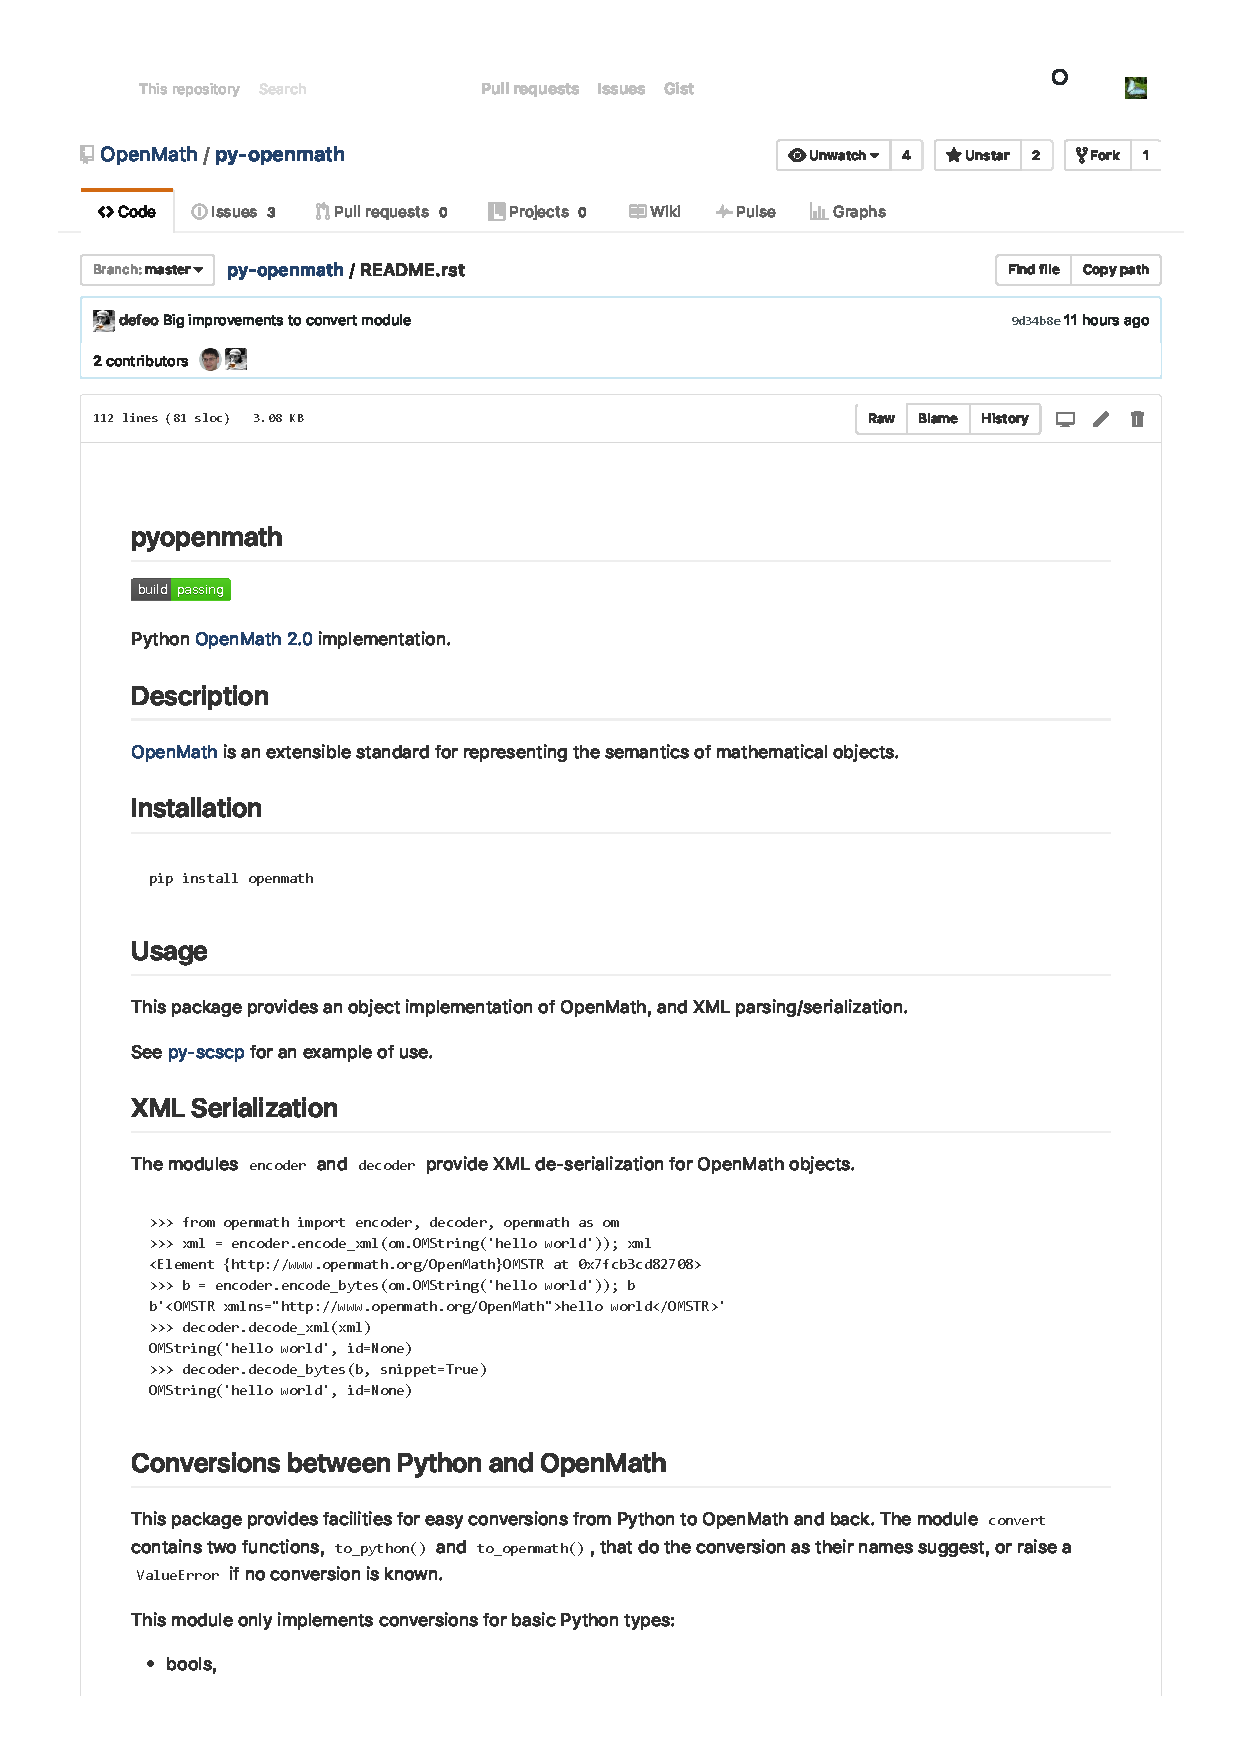
\includepdf[pages=-,scale=0.9,pagecommand={}]{READMEs/py-openmath_README.pdf}

\section{README file for the Python scscp package}\label{py-scscp_README}
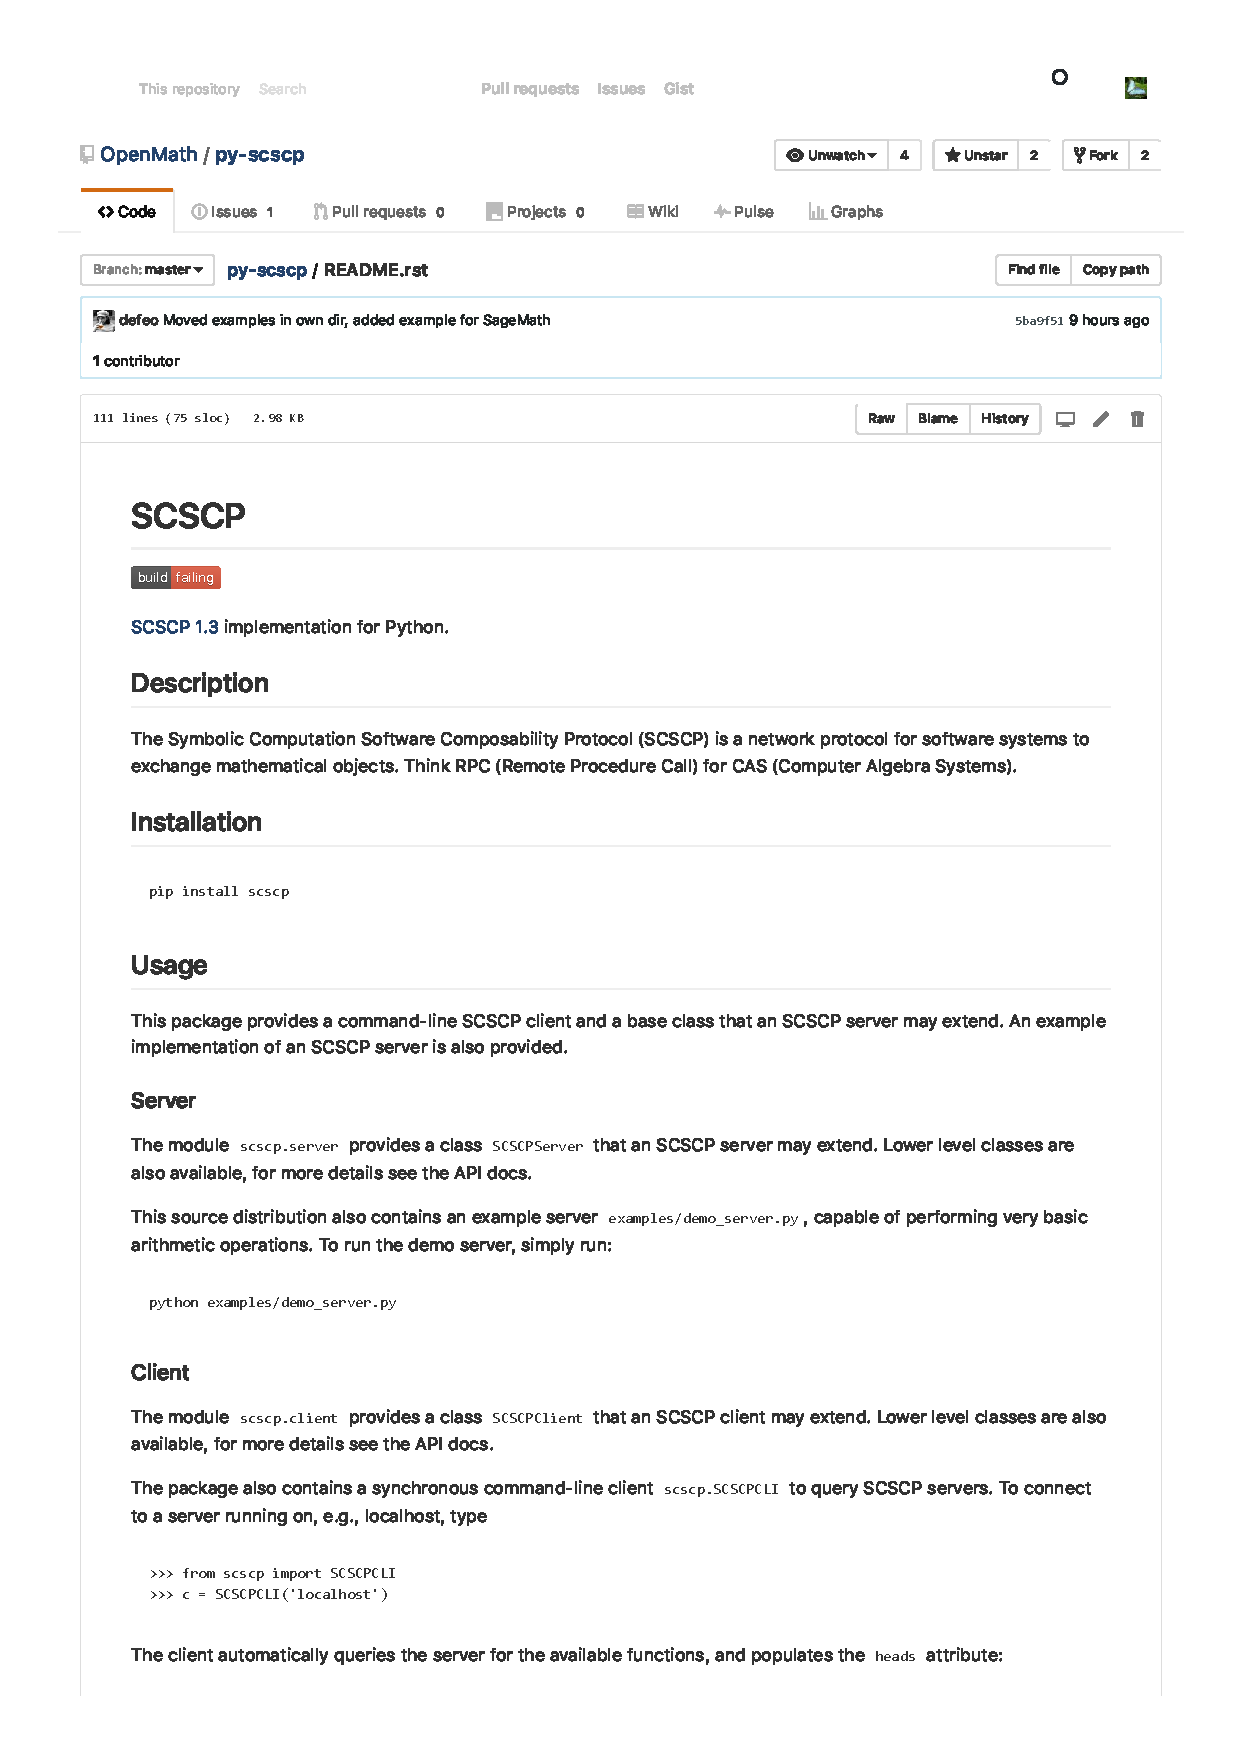
\includepdf[pages=-,scale=0.9,pagecommand={}]{READMEs/py-scscp_README.pdf}

\section{Example: SCSCP client in Python2 connecting to GAP server}\label{python2-to-GAP}
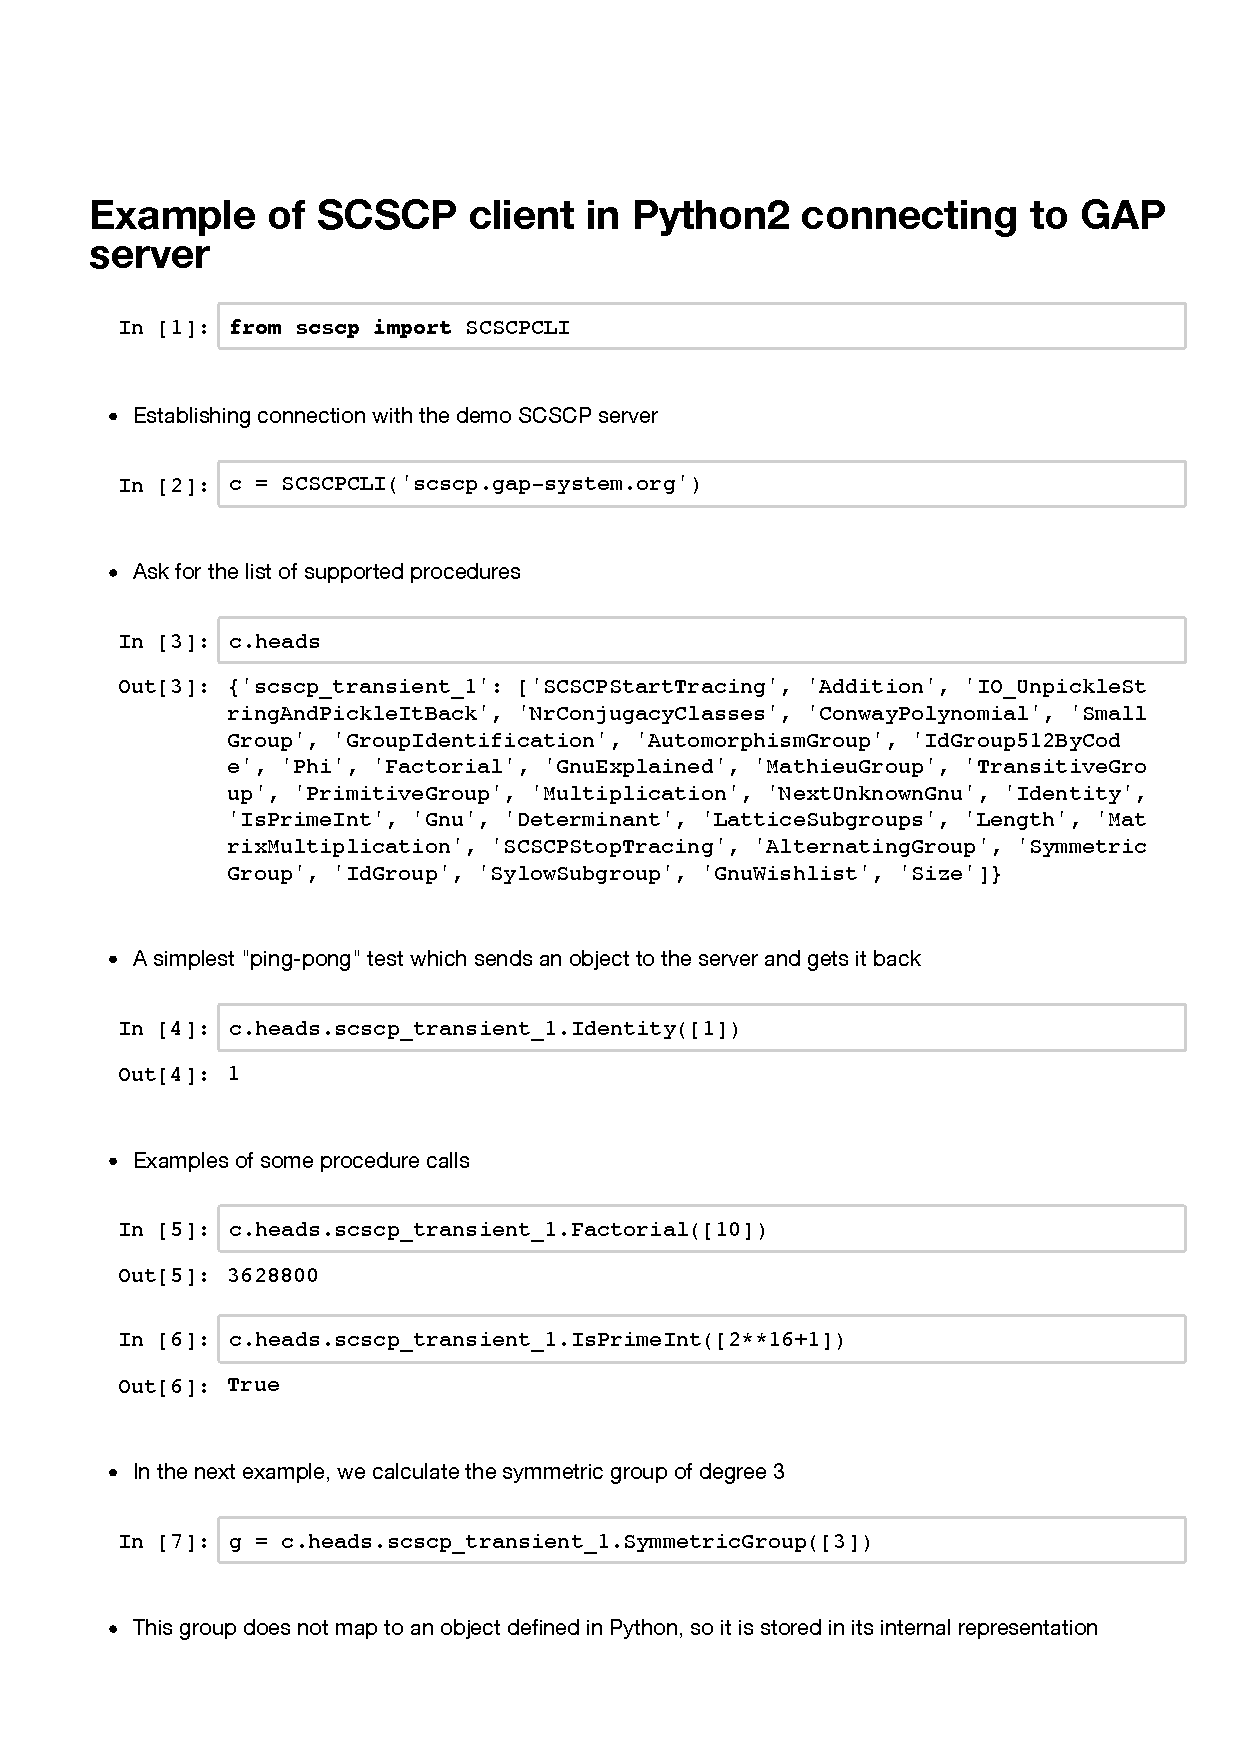
\includepdf[pages=-,scale=0.9,pagecommand={}]{examples/Python2-to-GAP.pdf}

\section{Example: SCSCP client in Python3 connecting to GAP server}\label{python3-to-GAP}
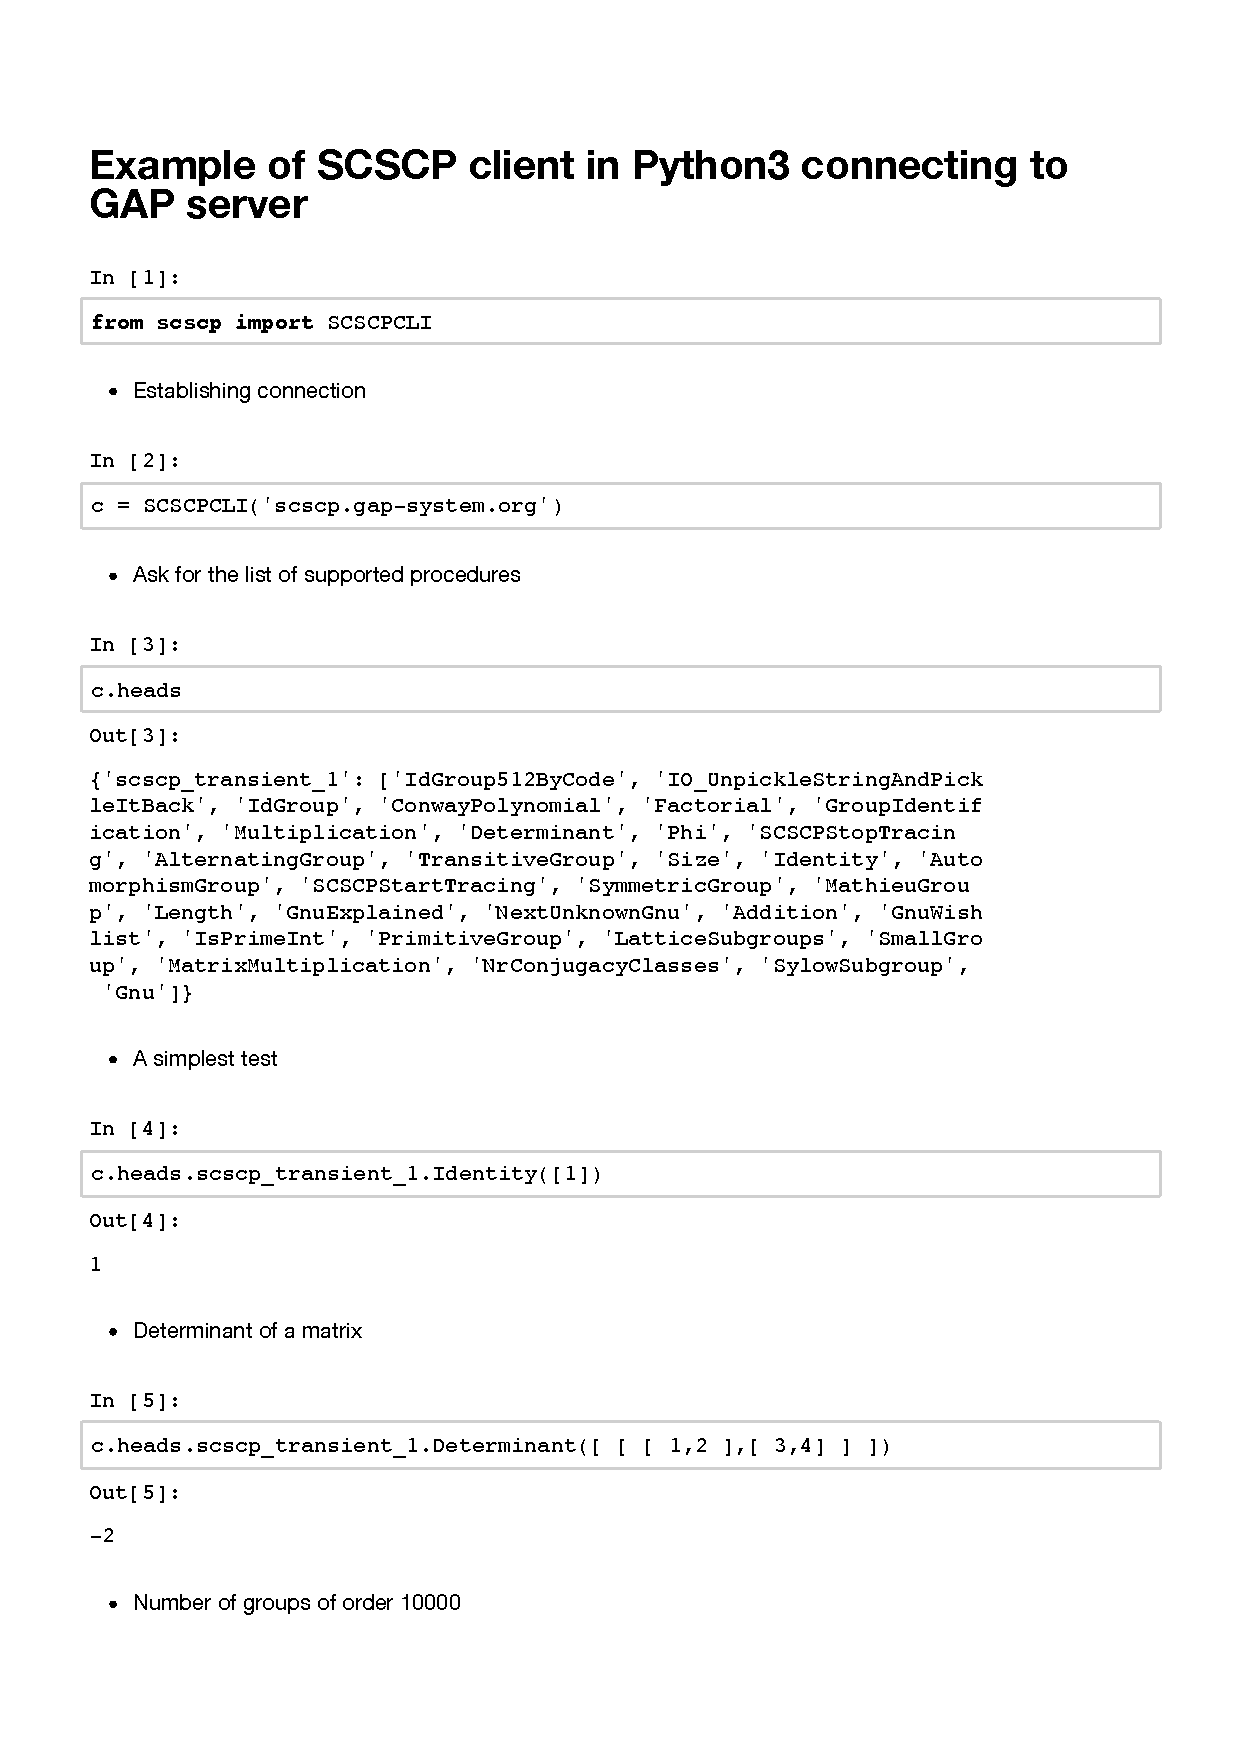
\includepdf[pages=-,scale=0.9,pagecommand={}]{examples/Python3-to-GAP.pdf}

\section{Example: SCSCP client in \Sage connecting to GAP server}\label{SageMath-to-GAP}
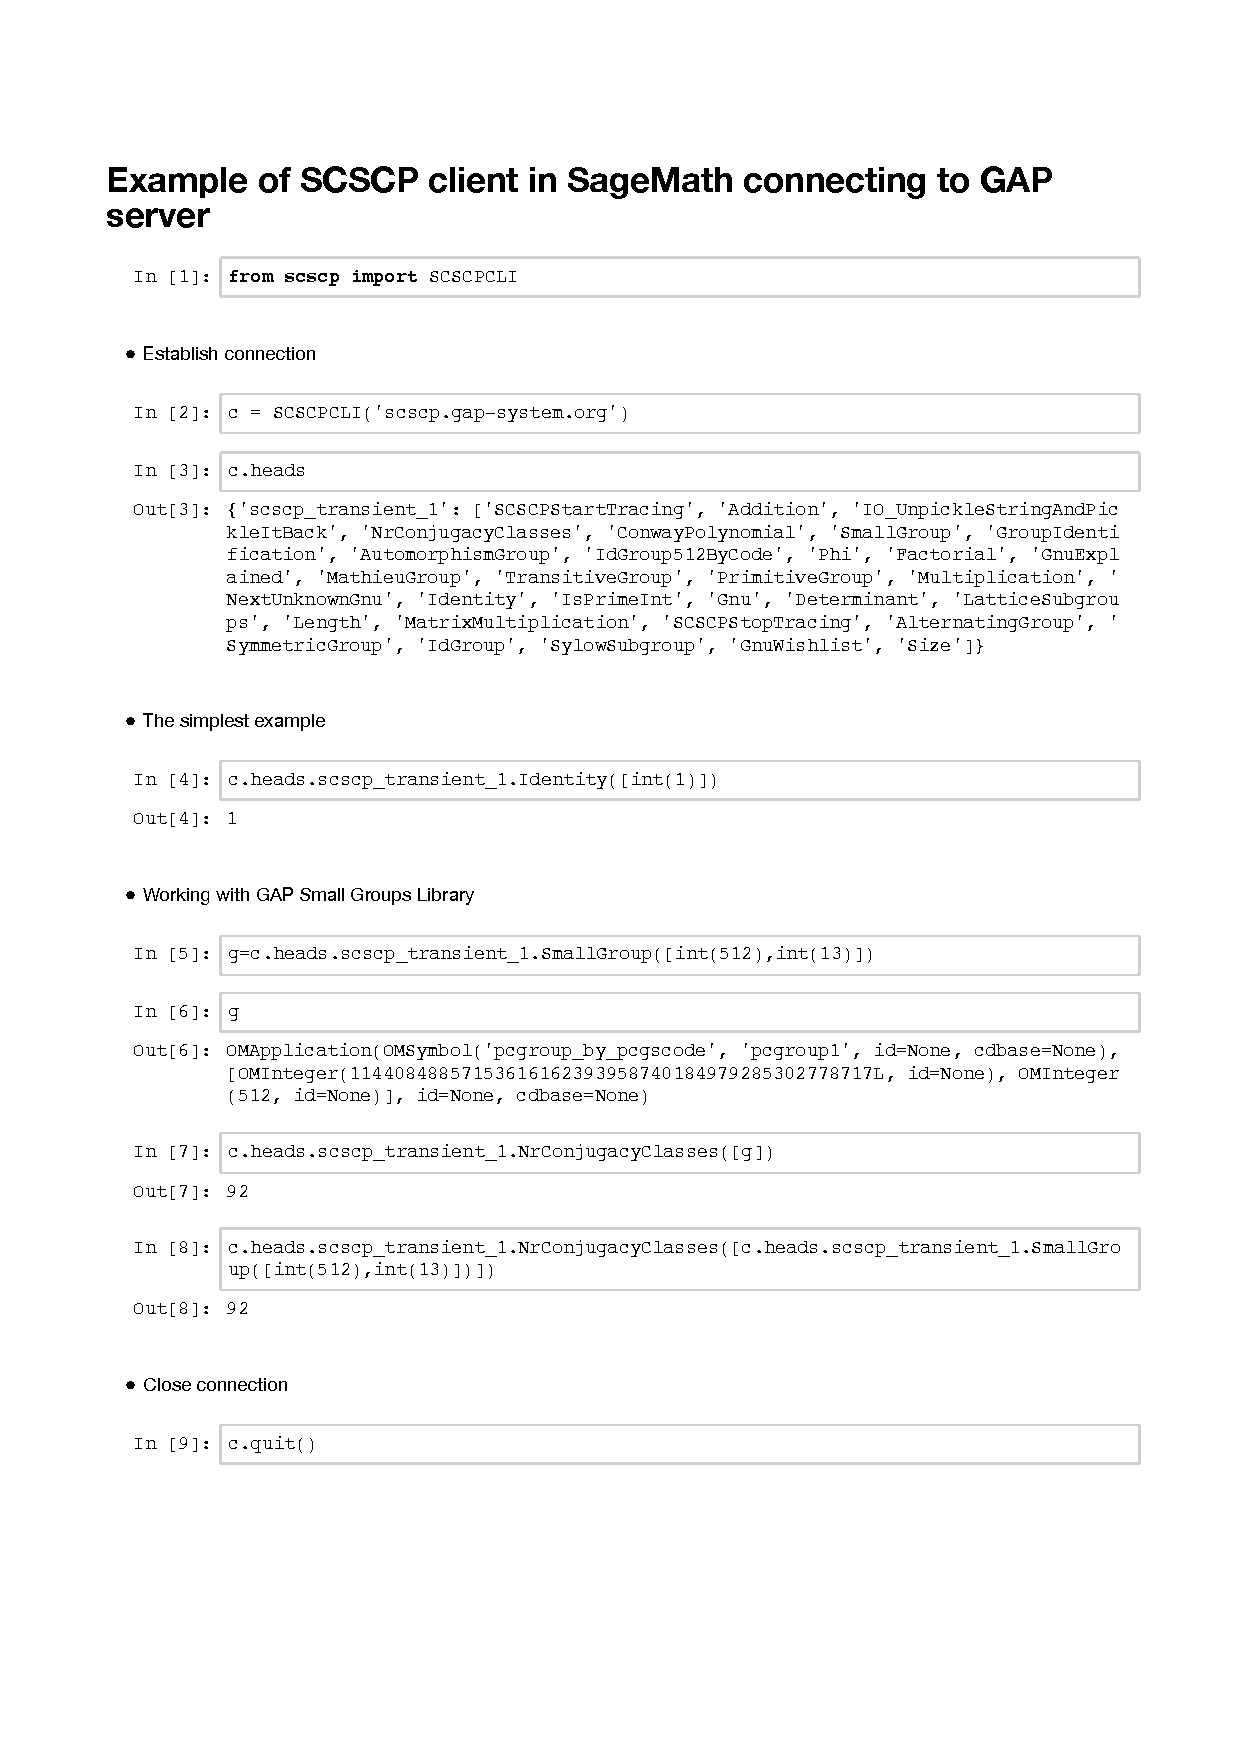
\includepdf[pages=-,scale=0.9,pagecommand={}]{examples/SageMath-to-GAP.pdf}

\section{Example: SCSCP client in Python3 calculates Groebner basis with \Singular}\label{Python3sympy-to-GAP-Singular}
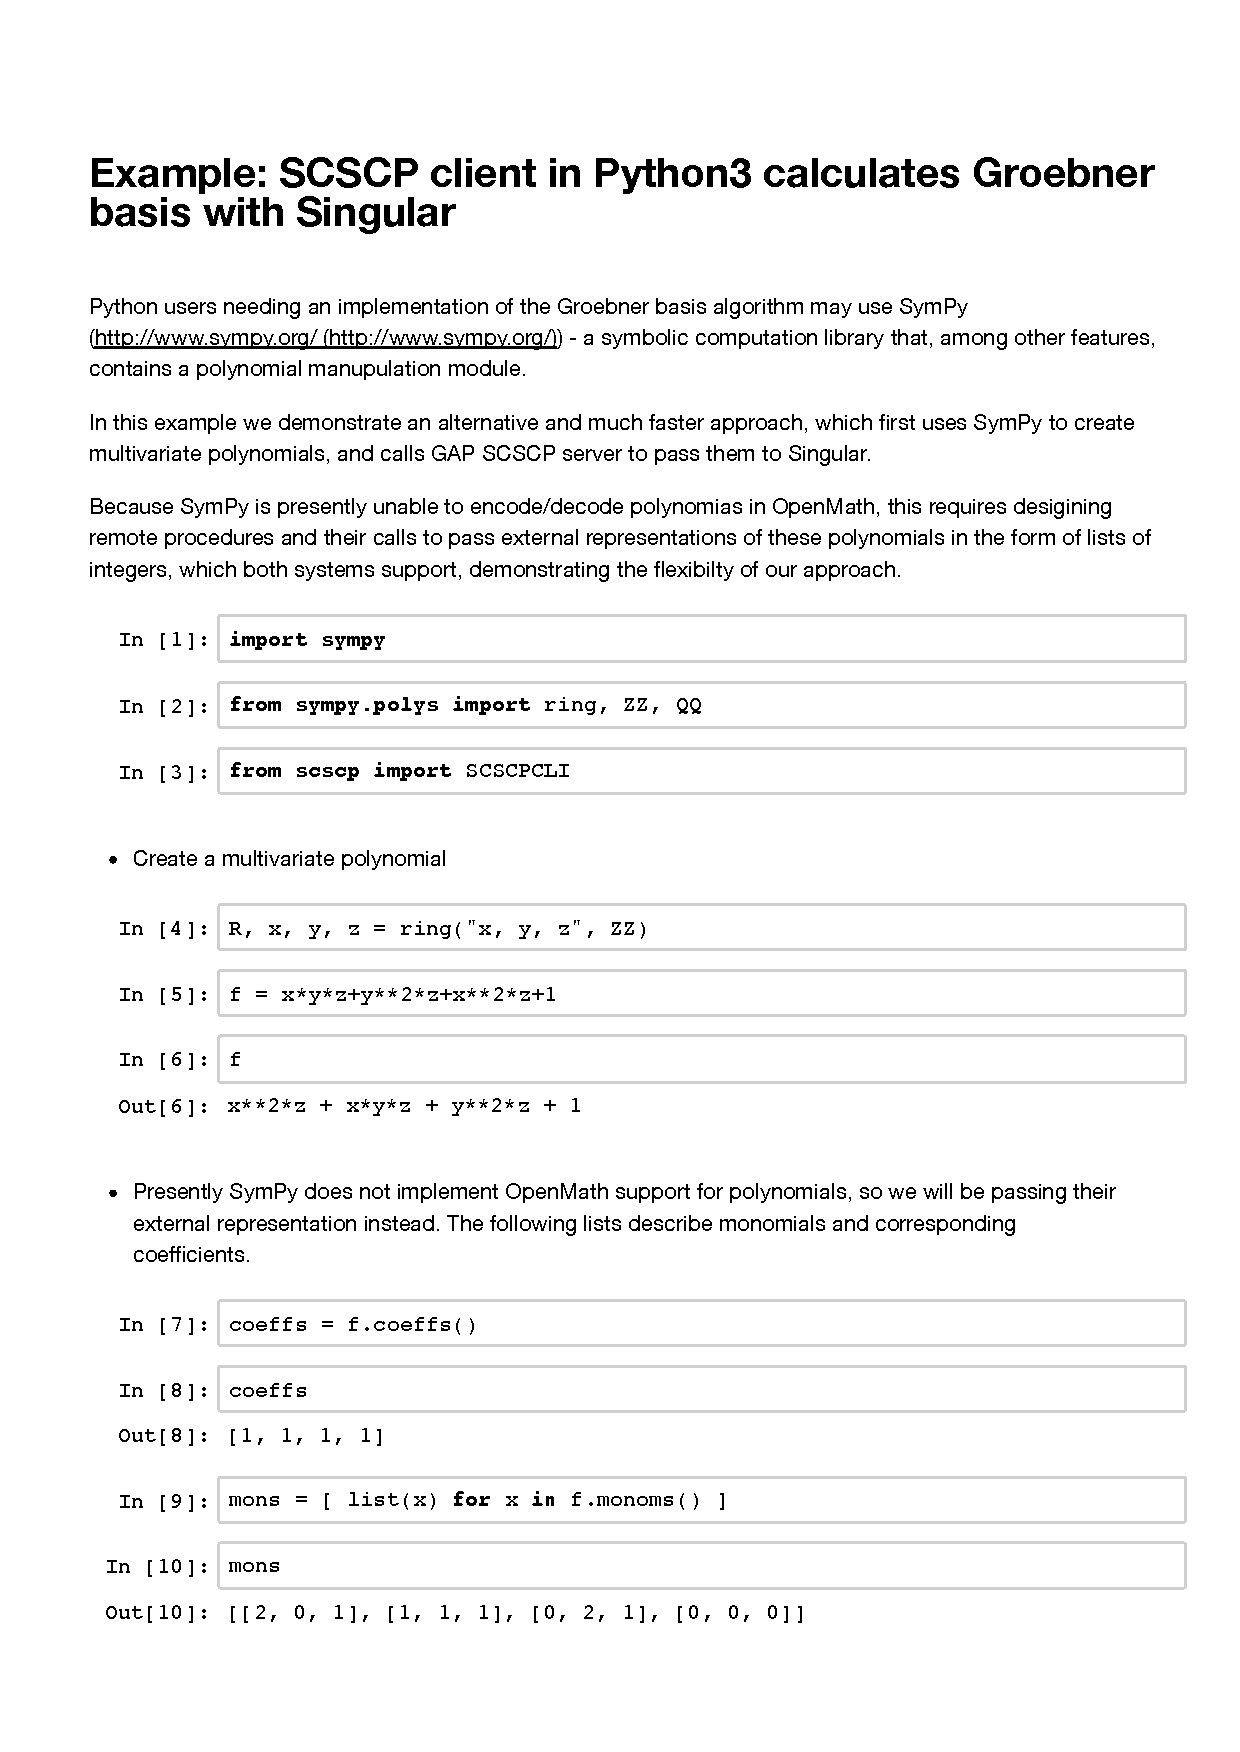
\includepdf[pages=-,scale=0.85,pagecommand={}]{examples/Python3sympy-to-GAP-Singular.pdf}
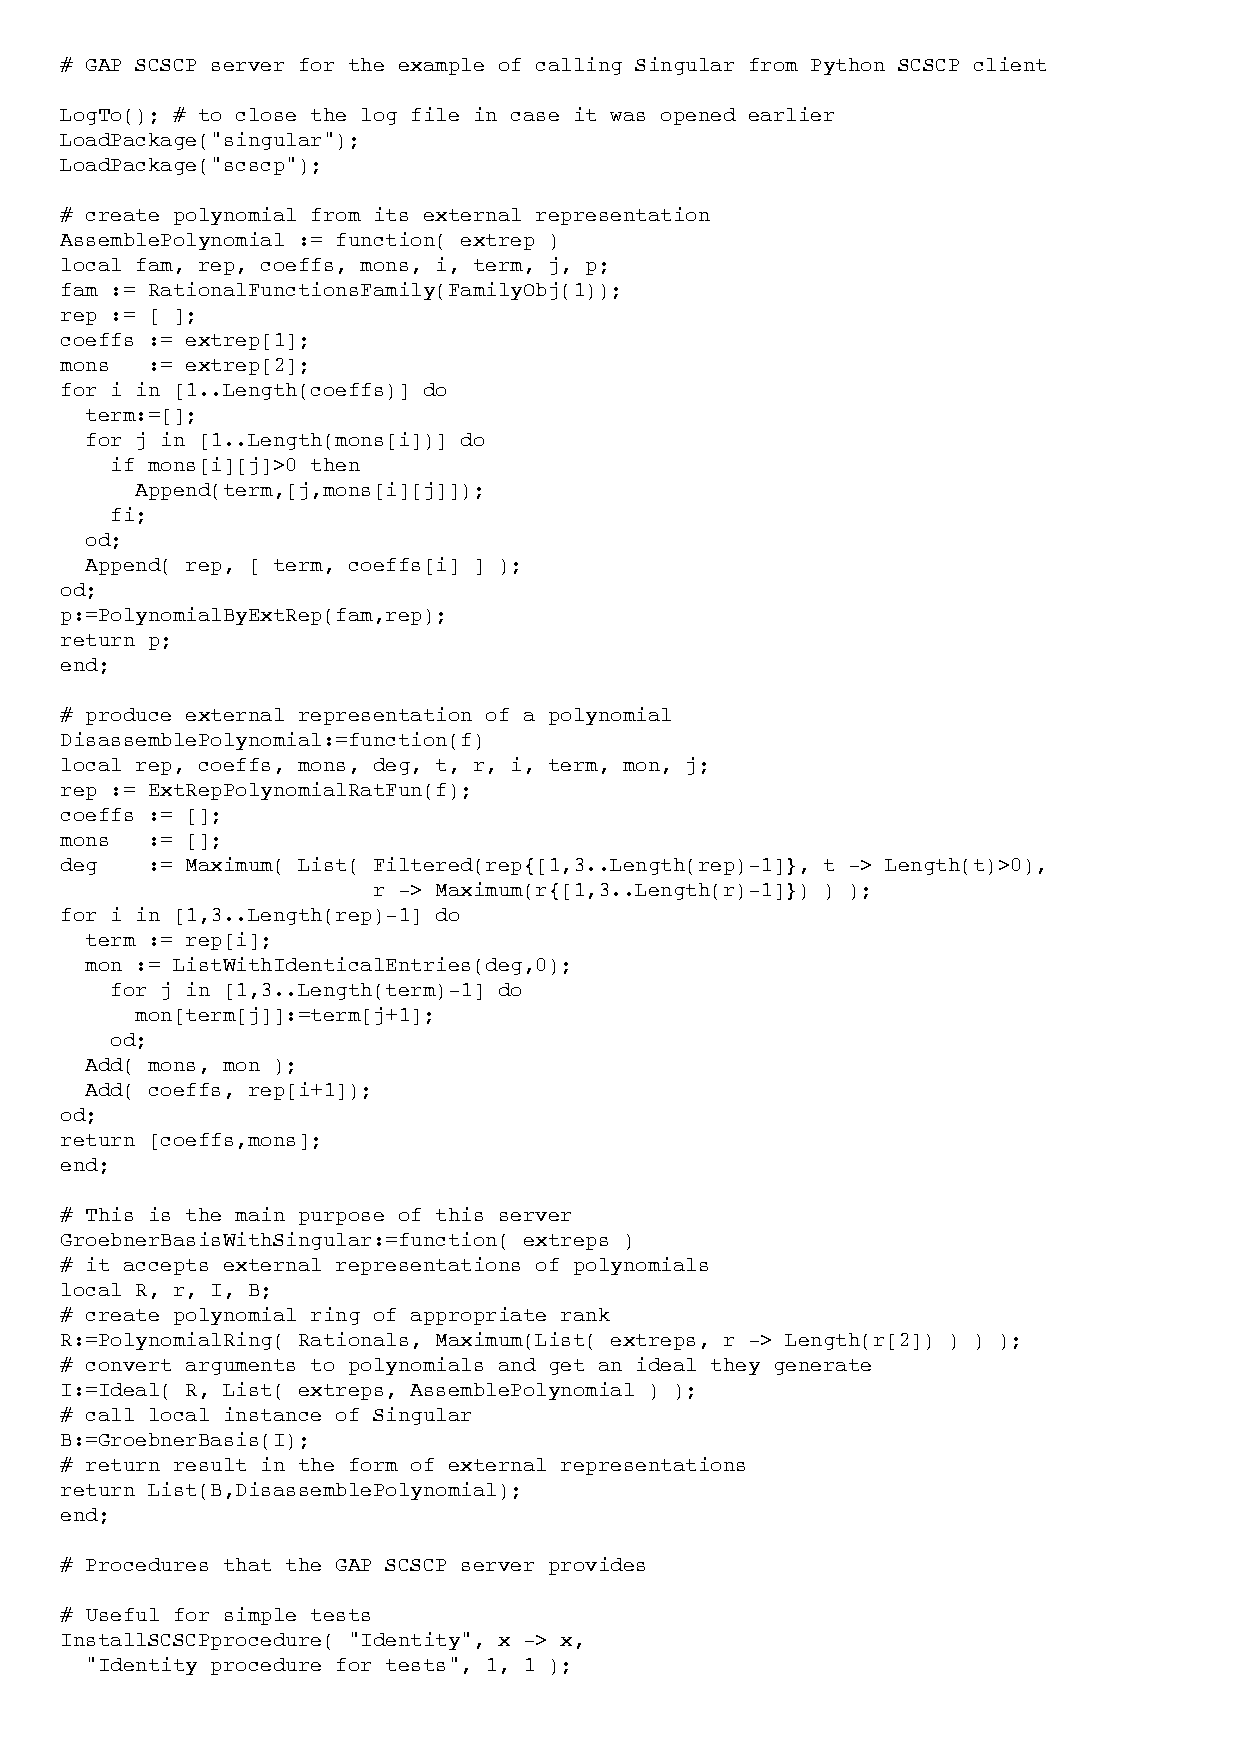
\includepdf[pages=-,scale=0.85,pagecommand={}]{examples/gap_singular_server.pdf}

\section{Example: SCSCP client in GAP connecting to Python 3 server}\label{GAP-to-Python3numpy}
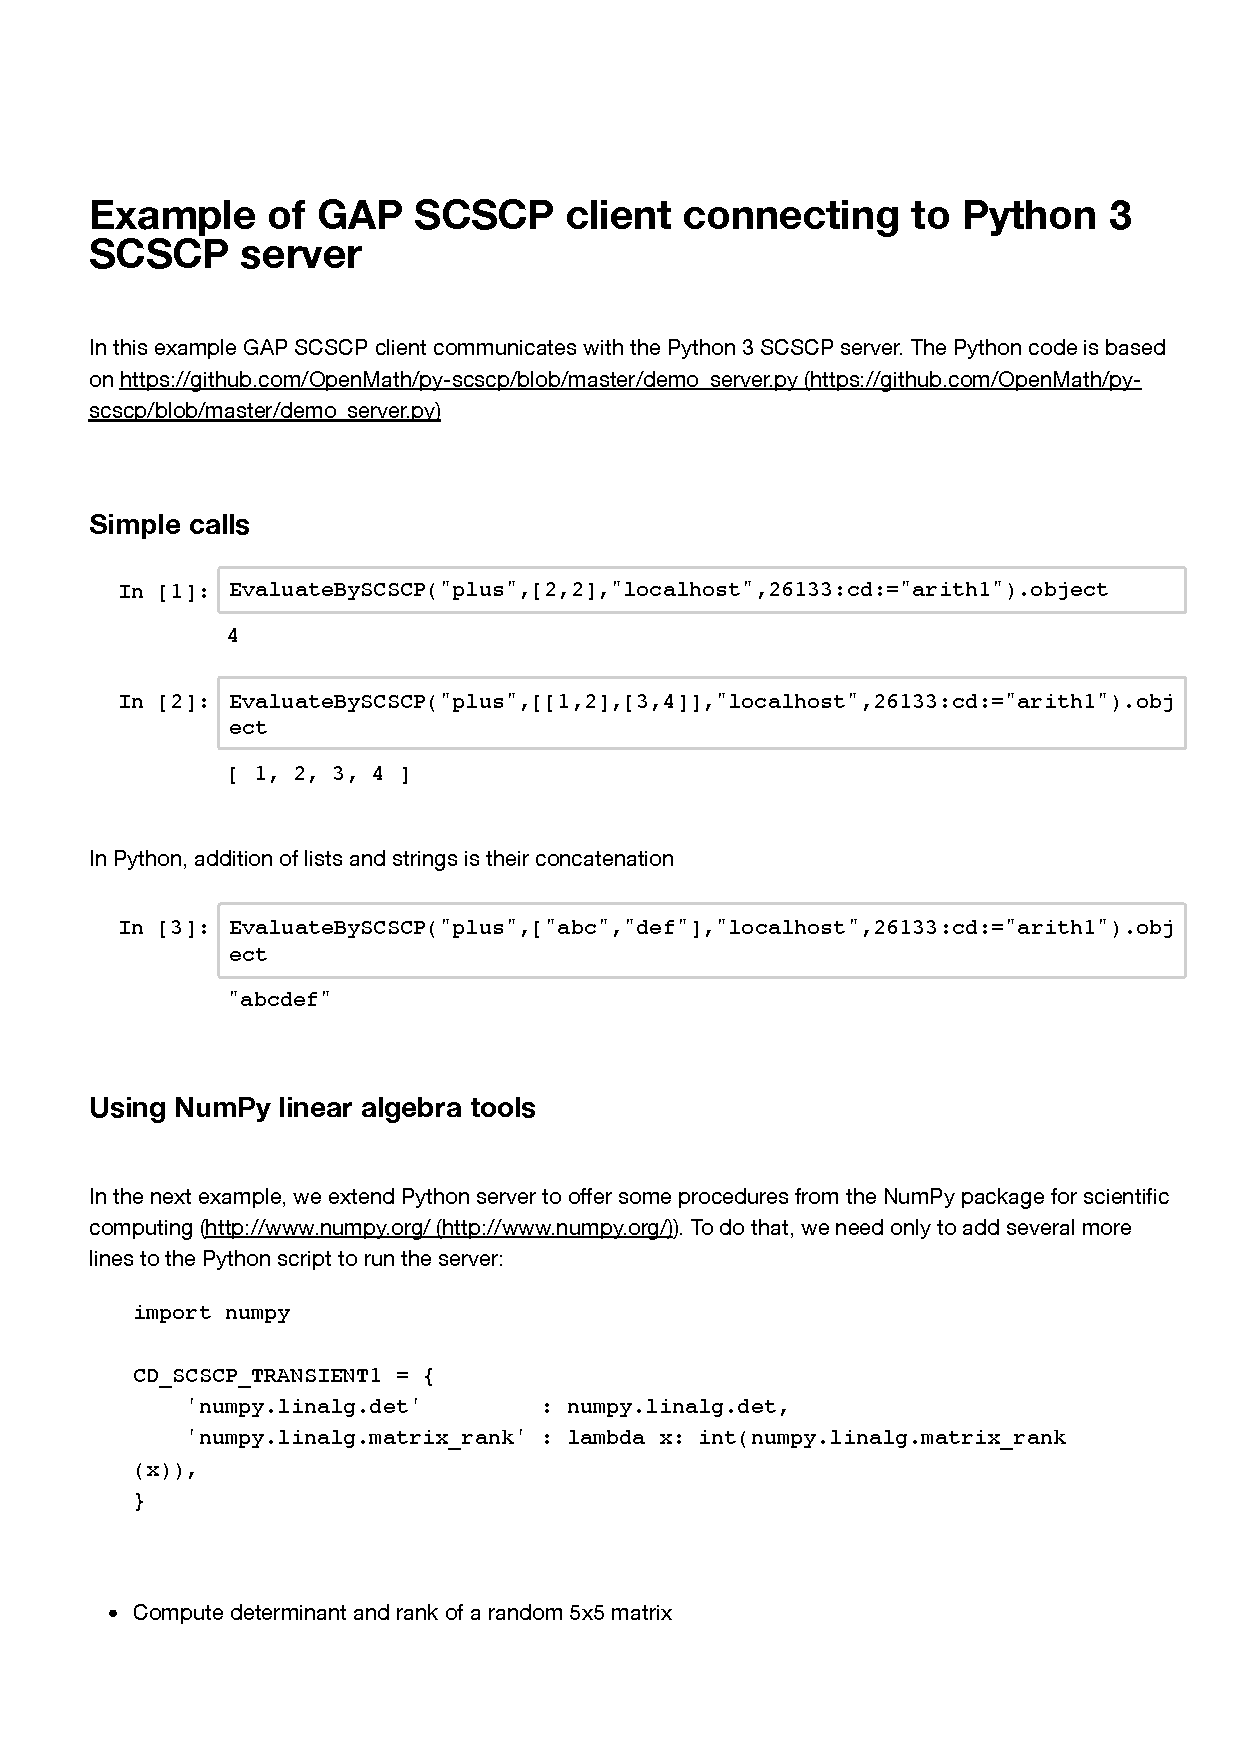
\includepdf[pages=-,scale=0.9,pagecommand={}]{examples/GAP-to-Python3numpy.pdf}

\section{Documentation for the GAP Docker container}\label{SCSCP-with-GAP-docker}
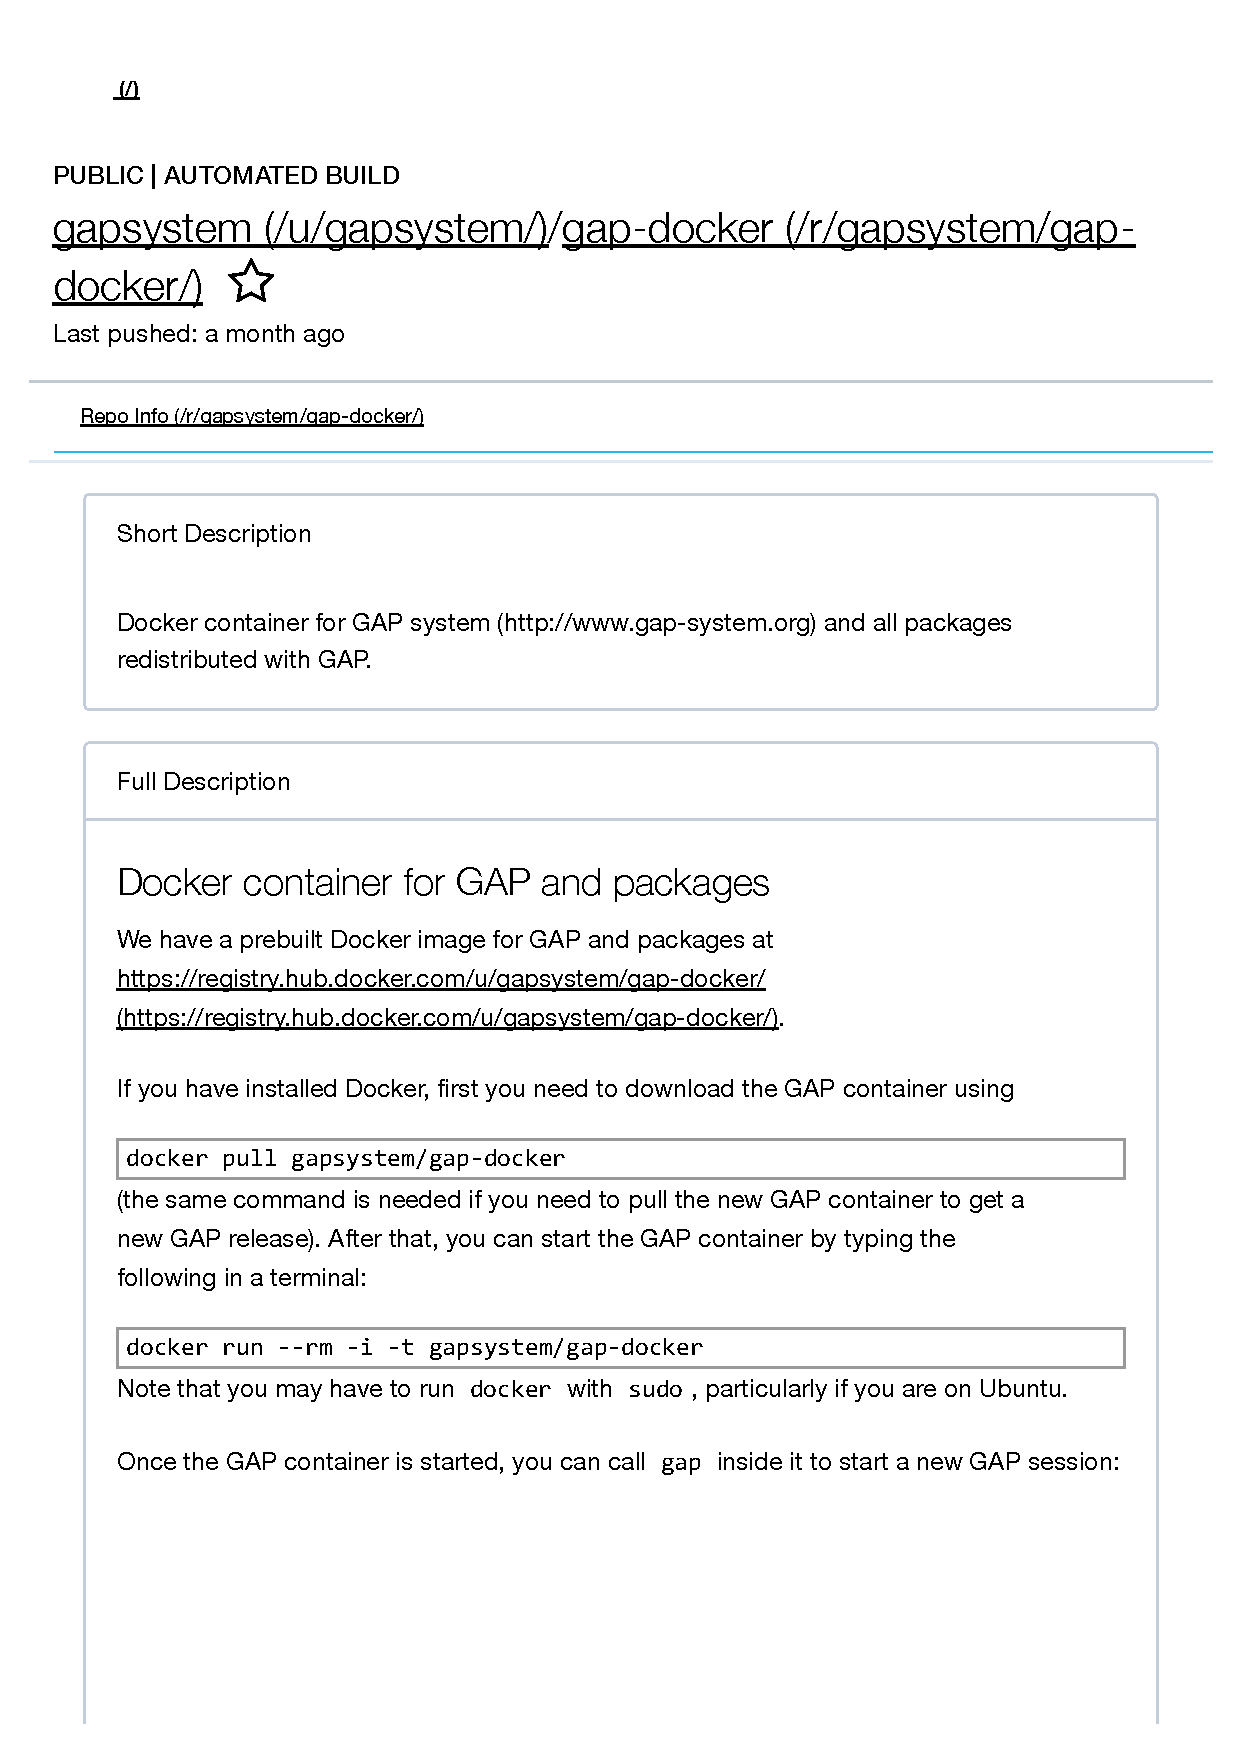
\includepdf[pages=-,scale=0.8,pagecommand={}]{READMEs/SCSCP-with-GAP-docker.pdf}

\section{Documentation for the GAP SCSCP server for the number of isomorphism types of groups of order $n$}\label{Gnu-SCSCP-server}
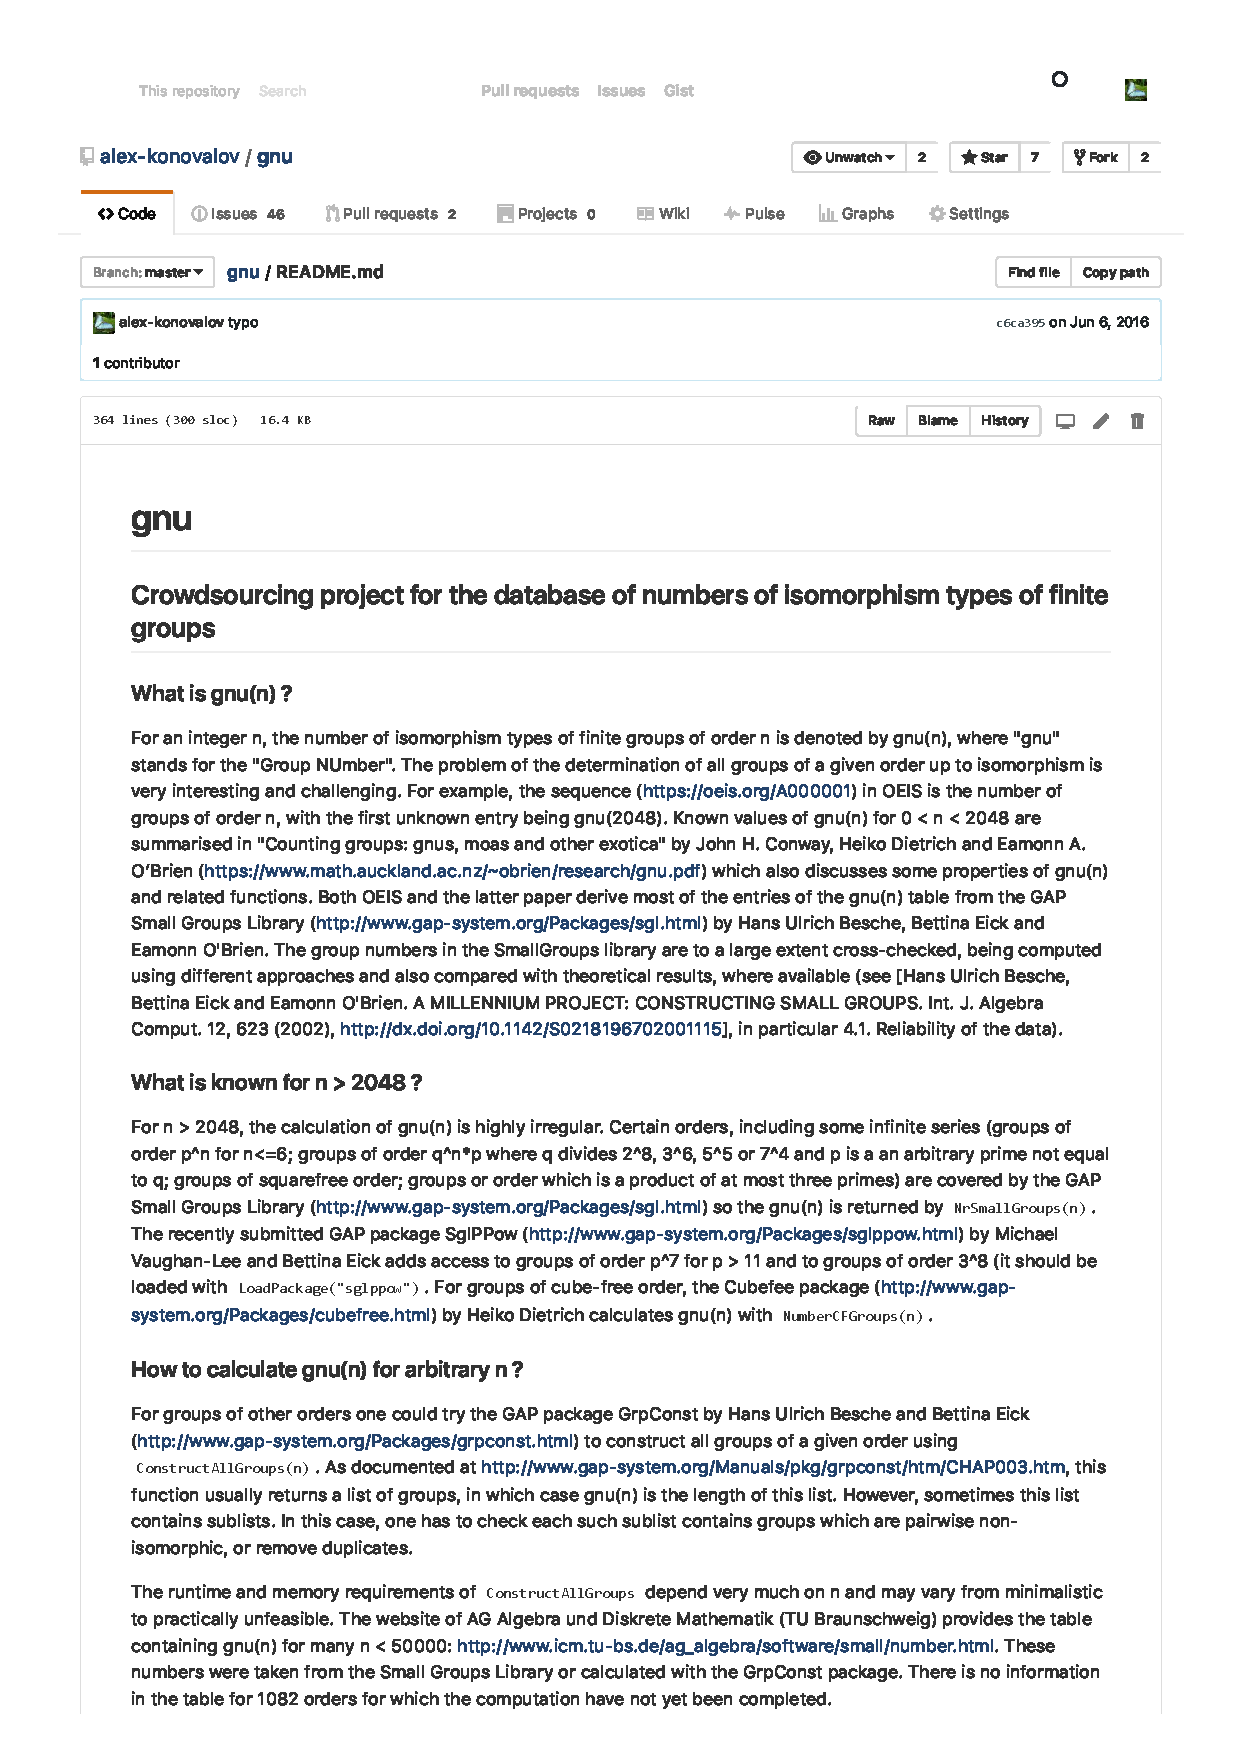
\includepdf[pages=-,scale=0.9,pagecommand={}]{READMEs/Gnu-SCSCP-server.pdf}

\section{Parallel search in the GAP Small Groups Library with SCSCP}
\label{Parallel-GAP-SCSCP}
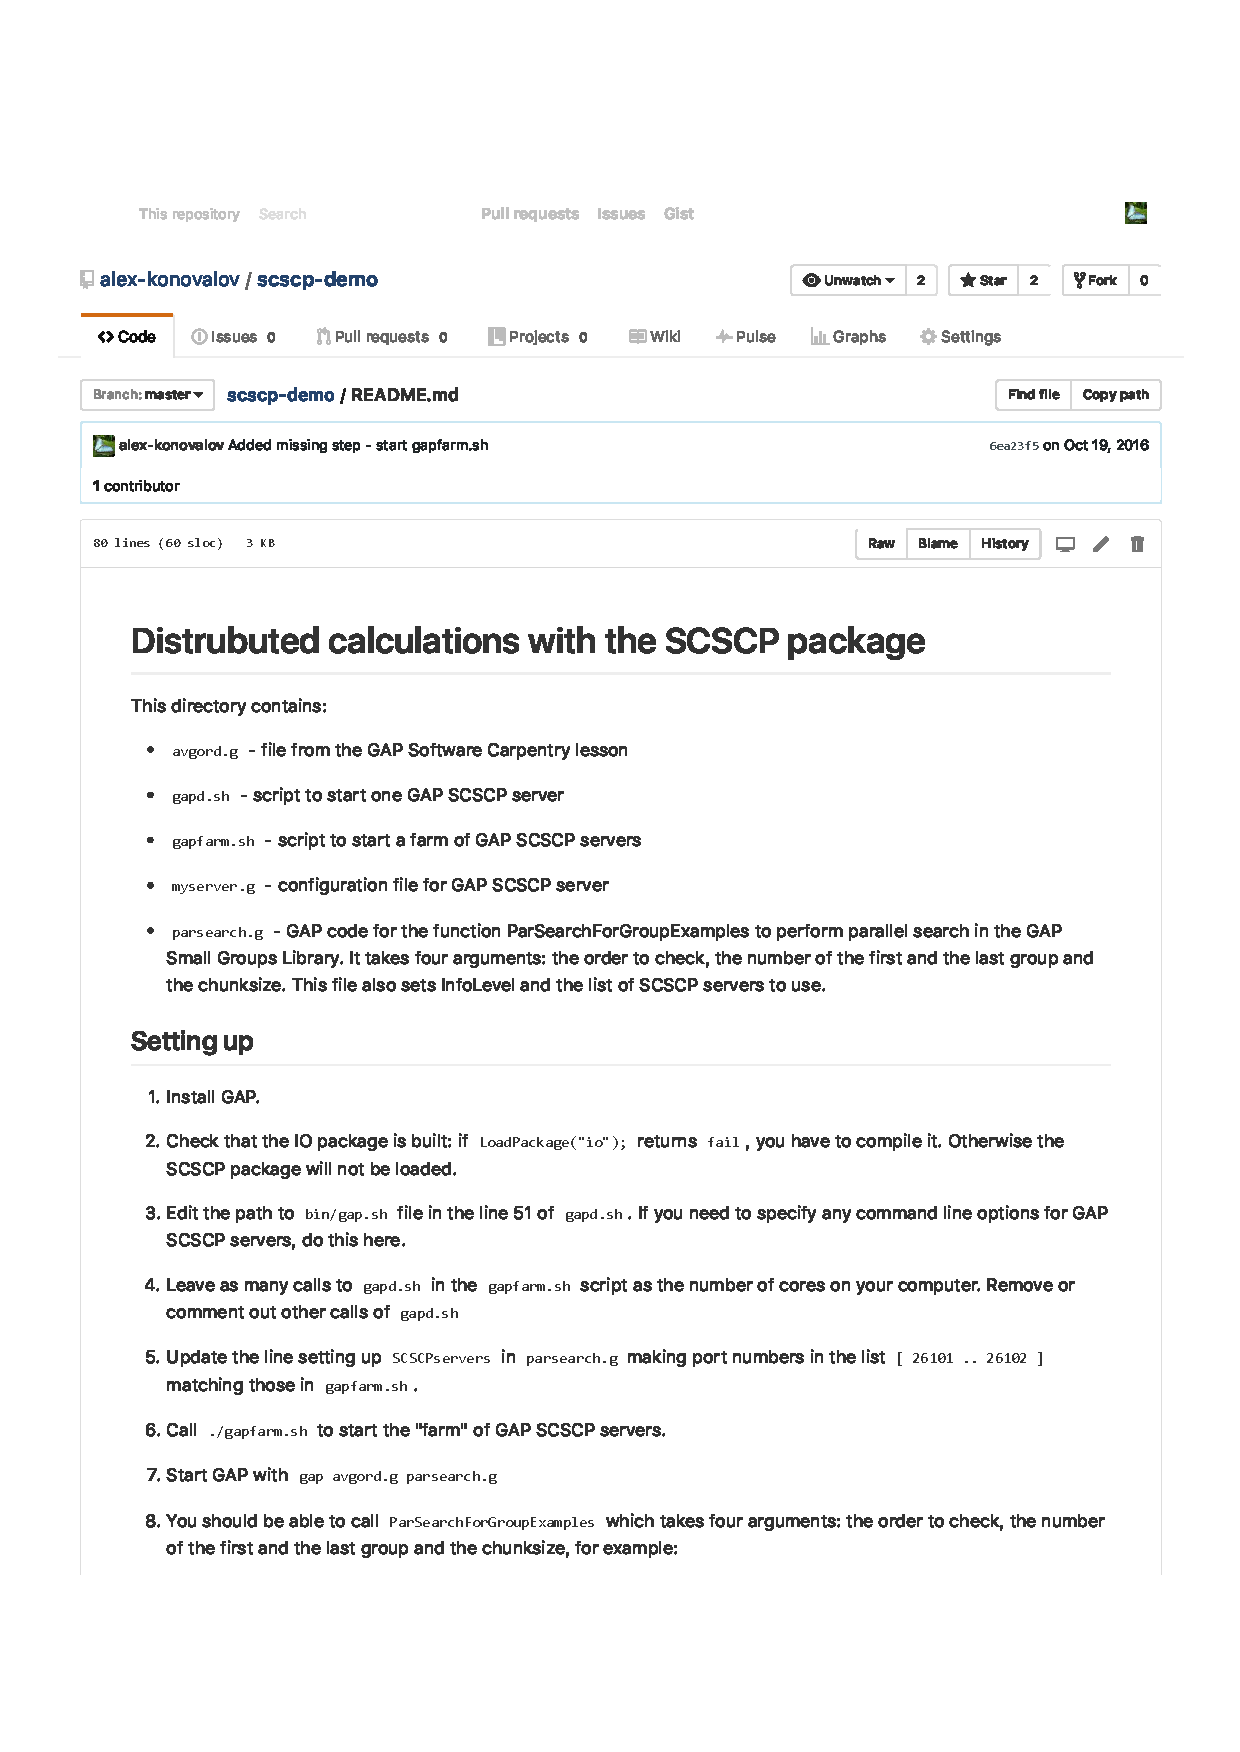
\includepdf[pages=-,scale=0.9,pagecommand={}]{READMEs/Parallel-GAP-SCSCP.pdf}

\section{Example: SCSCP Client from within  Scala}
\label{mmt-simple-example-SCSCP}
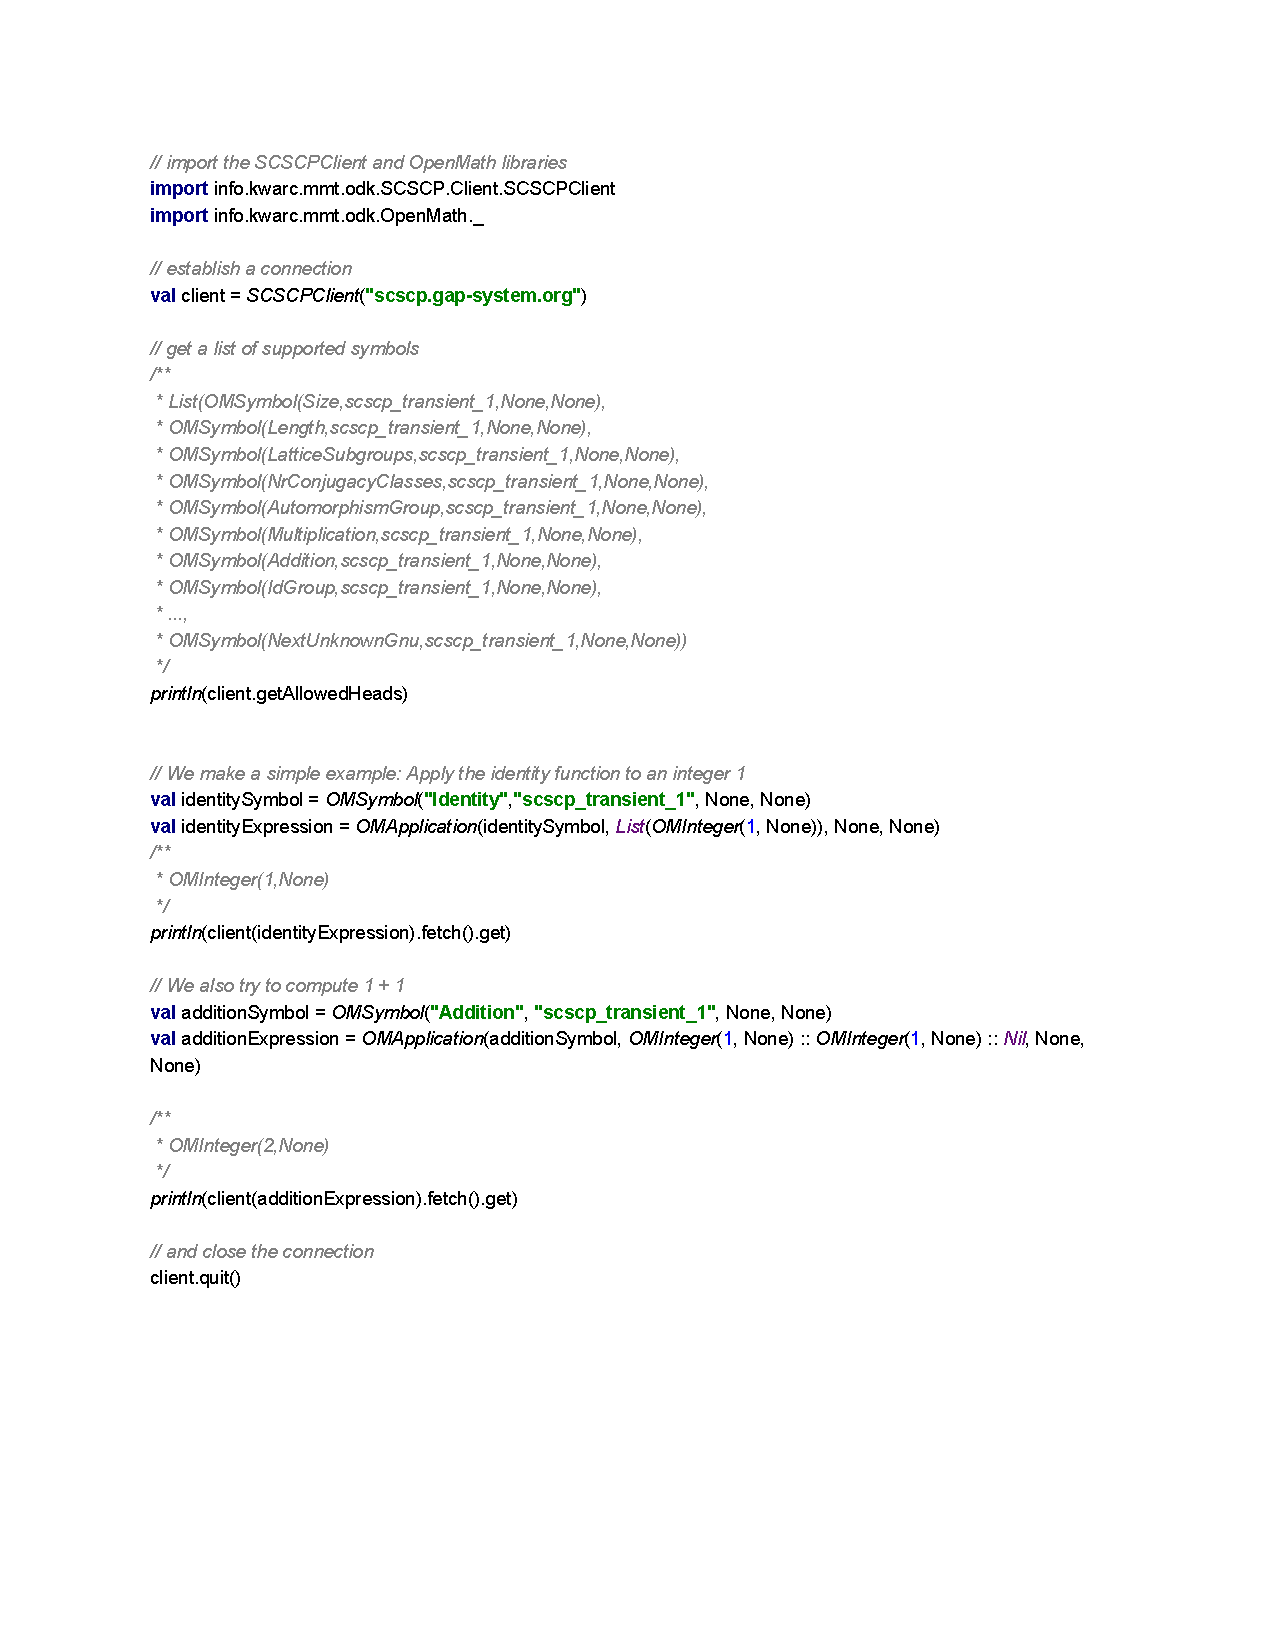
\includepdf[pages=-,scale=0.9,pagecommand={}]{examples/MMT_simple_client_example.pdf}

%\section{Example: SCSCP Client from within MMT}
%\label{mmt-advanced-example}
%TODO: Finish this example

\end{document}

%%% Local Variables:
%%% mode: latex
%%% TeX-master: t
%%% End:

%  LocalWords:  githubissuedescription newpage tableofcontents newpage printbibliography
